\chapter{Uczenie modelu detekcji choroby Alzheimera oraz jego wykorzystanie}

W tej pracy chcę przedstawić możliwości wykorzystania bibliotek uczenia maszynowego w środowisku \emph{.NET} w celu uczenia oraz późniejszego wykorzystania modelu głębokiej sieci neuronowej do detekcji choroby Alzheimera oraz stopnia demencji na obrazach rezonansu magnetycznego mózgów pacjentów, a także postaram się je porównać między sobą oraz z istniejącymi rozwiązaniami także spoza środowiska \emph{.NET}.

\section{Zbiór danych}

Wykorzystany zbiór pochodzi z platformy Kaggle (udostępniony jest pod adresem \url{kaggle.com/datasets/tourist55/alzheimers-dataset-4-class-of-images}, zapewniony na podstawie licencji \emph{Open Data Commons Open Database License} (\emph{ODbL}) wersji $1.0$) \cite{kaggle-alzheimers-dataset}.
Jest wstępnie podzielony na zbiór treningowy oraz testowy w celu zapewnienia powtarzalności i porównywalności wyników uzyskanych z użyciem różnych narzędzi i z różnych źródeł.
Zawiera on zestaw obrazów uzyskanych z badań rezonansem magnetycznym (MRI), których celem jest analiza i diagnoza otępienia spowodowanego chorobą Alzheimera.
Obrazy te są dwuwymiarowym wycinkiem trójwymiarowego skanu rezonansu magnetycznego mózgu, który najlepiej obrazuje strukturę mózgu i potencjalne zmiany chorobowe.
Mają wymiary $208 \times 176$ pikseli -- wystarczająco duże, aby widoczne były nawet drobne detale ale na tyle małe, aby były możliwe do przetworzenia przez mniejsze sieci neuronowe a także umożliwiły ich znacznie szybsze szkolenie.

Zbiór danych składa się z czterech kategorii obrazów, zarówno w zbiorze treningowym, jak i testowym:

\begin{itemize}

  \item
        Brak demencji (\emph{Non Demented}) -- ta kategoria zawiera obrazy mózgów osób niebędących dotkniętymi demencją.
        W zbiorze treningowym znajduje się 2560 obrazów, a w zbiorze testowym 640 obrazów, co daje sumarycznie 3200 zdjęć z tej kategorii.

  \item
        Bardzo łagodna demencja (\emph{Very Mild Demented}) -- zbiór ten obejmuje obrazy osób z bardzo łagodnym stopniem demencji.
        W zbiorze treningowym znajduje się 1792 obrazy, a w zbiorze testowym 448 obrazów, co daje łącznie 2240 obrazów z tej kategorii.

  \item
        Łagodna demencja (\emph{Mild Demented}) -- ten zbiór zawiera obrazy mózgów pacjentów cierpiących na łagodne otępienie związanego z chorobą Alzheimera.
        W zbiorze treningowym znajduje się 717 obrazów, a w zbiorze testowym 179 obrazów, co daje łączną sumę 896 obrazów z tej kategorii.

  \item
        Umiarkowana demencja (\emph{Moderate Demented}) -- ta kategoria obejmuje obrazy mózgów pacjentów już z wyższym stopniem demencji związanym z chorobą Alzheimera.
        W zbiorze treningowym znajduje się 52 obrazy, a w zbiorze testowym 12 obrazów, co daje łącznie 64 obrazy z tej kategorii.

\end{itemize}

\begin{figure}[ht]
  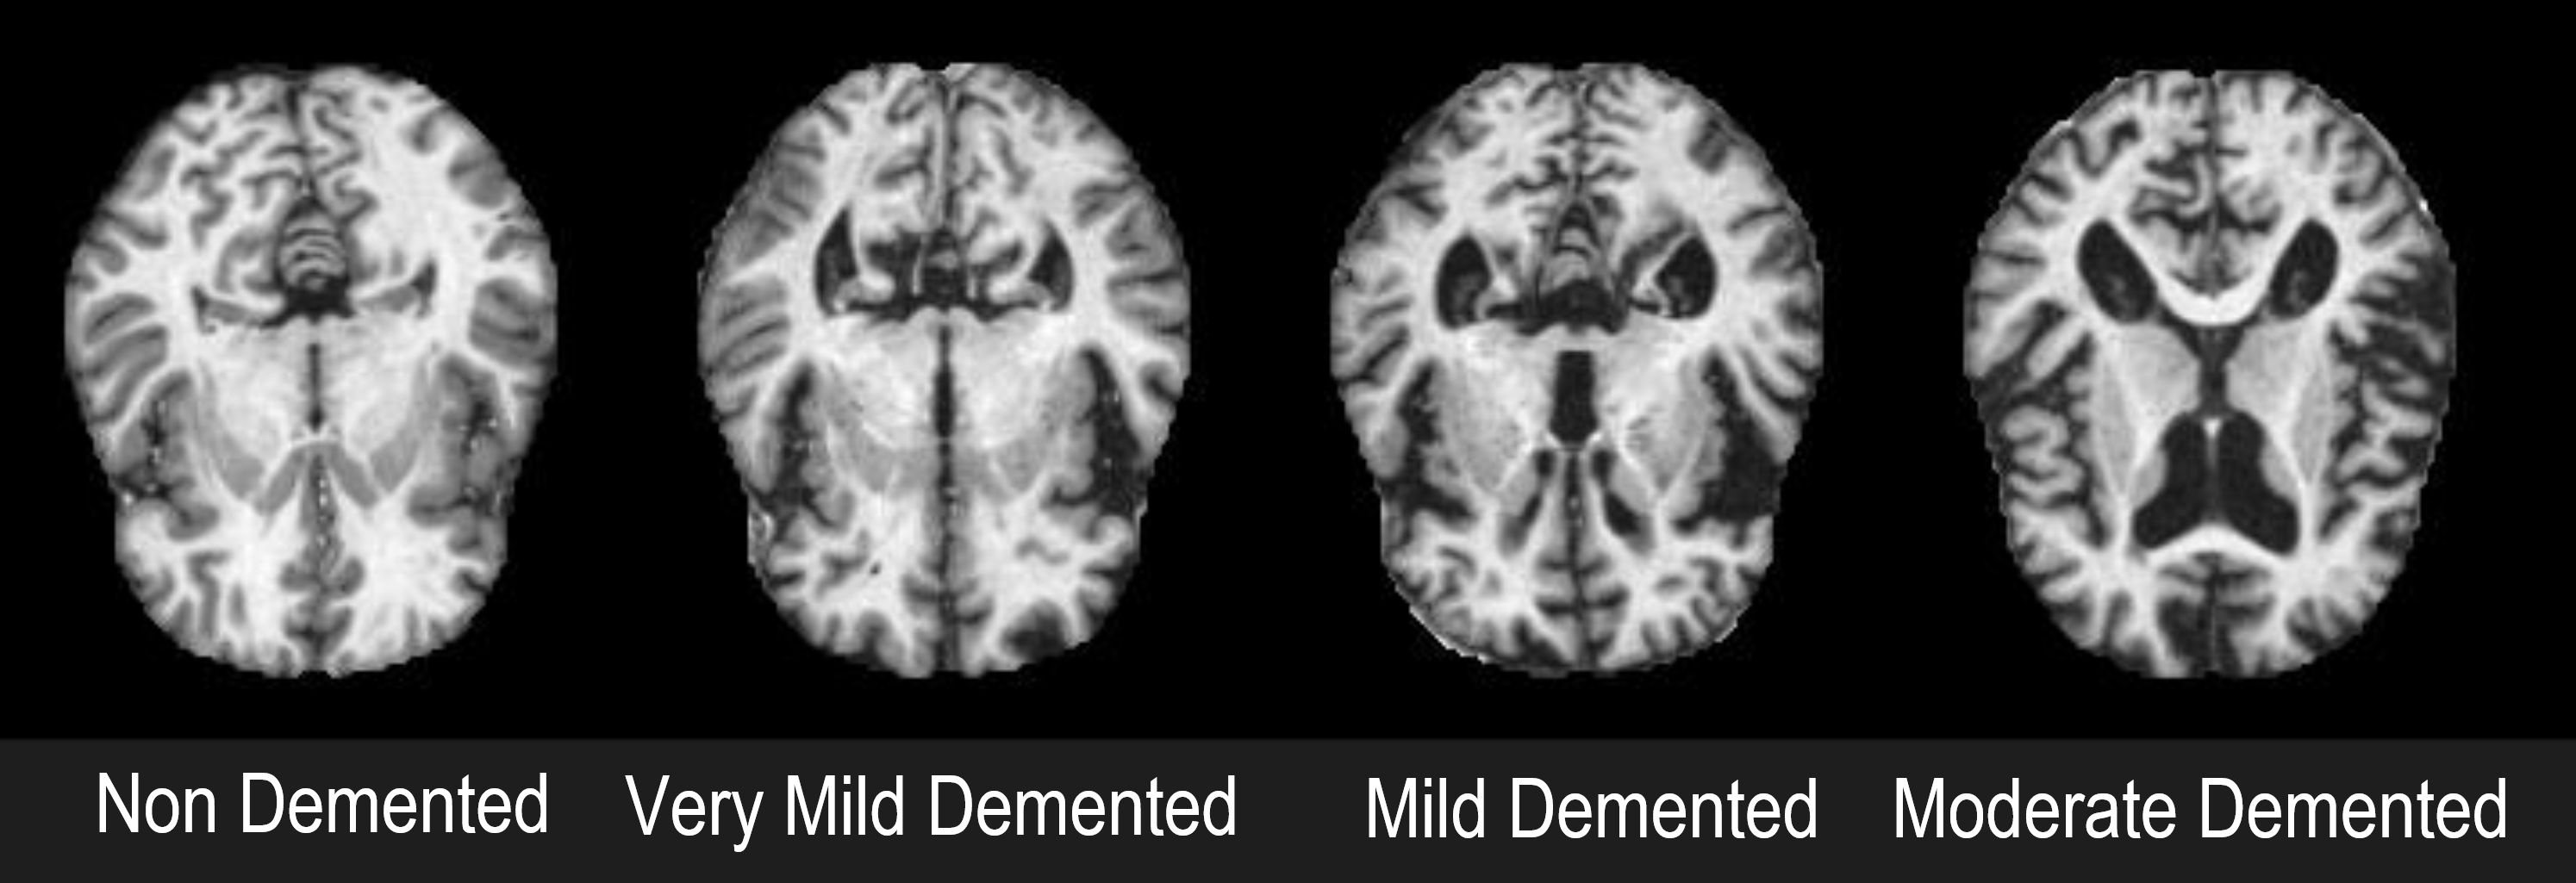
\includegraphics[width=\textwidth]{dataset-image-examples}
  \caption[Zestawienie przykładowych obrazów z każdej kategorii zbioru danych]{Zestawienie przykładowych obrazów z każdej kategorii zbioru danych \cite{kaggle-alzheimers-dataset}, gdzie przedstawione od lewej są: obraz mózgu osoby bez demencji, obraz mózgu osoby z bardzo lekką demencją, obraz mózgu osoby z lekką demencją o podłożach w chorobie Alzheimera oraz obraz mózgu osoby z umiarkowaną demencją chorą na Alzheimera.}
  \label{fig:dataset-image-examples}
\end{figure}

Przykłady obrazów z poszczególnych kategorii przedstawione są na \hyperref[fig:dataset-image-examples]{rysunku \ref*{fig:dataset-image-examples}}.

\section{Uczenie modelu z użyciem narzędzia ML.NET}

\subsection{Uczenie modelu z wykorzystaniem niestandardowego kodu biblioteki ML.NET}

\begin{figure}[ht]
  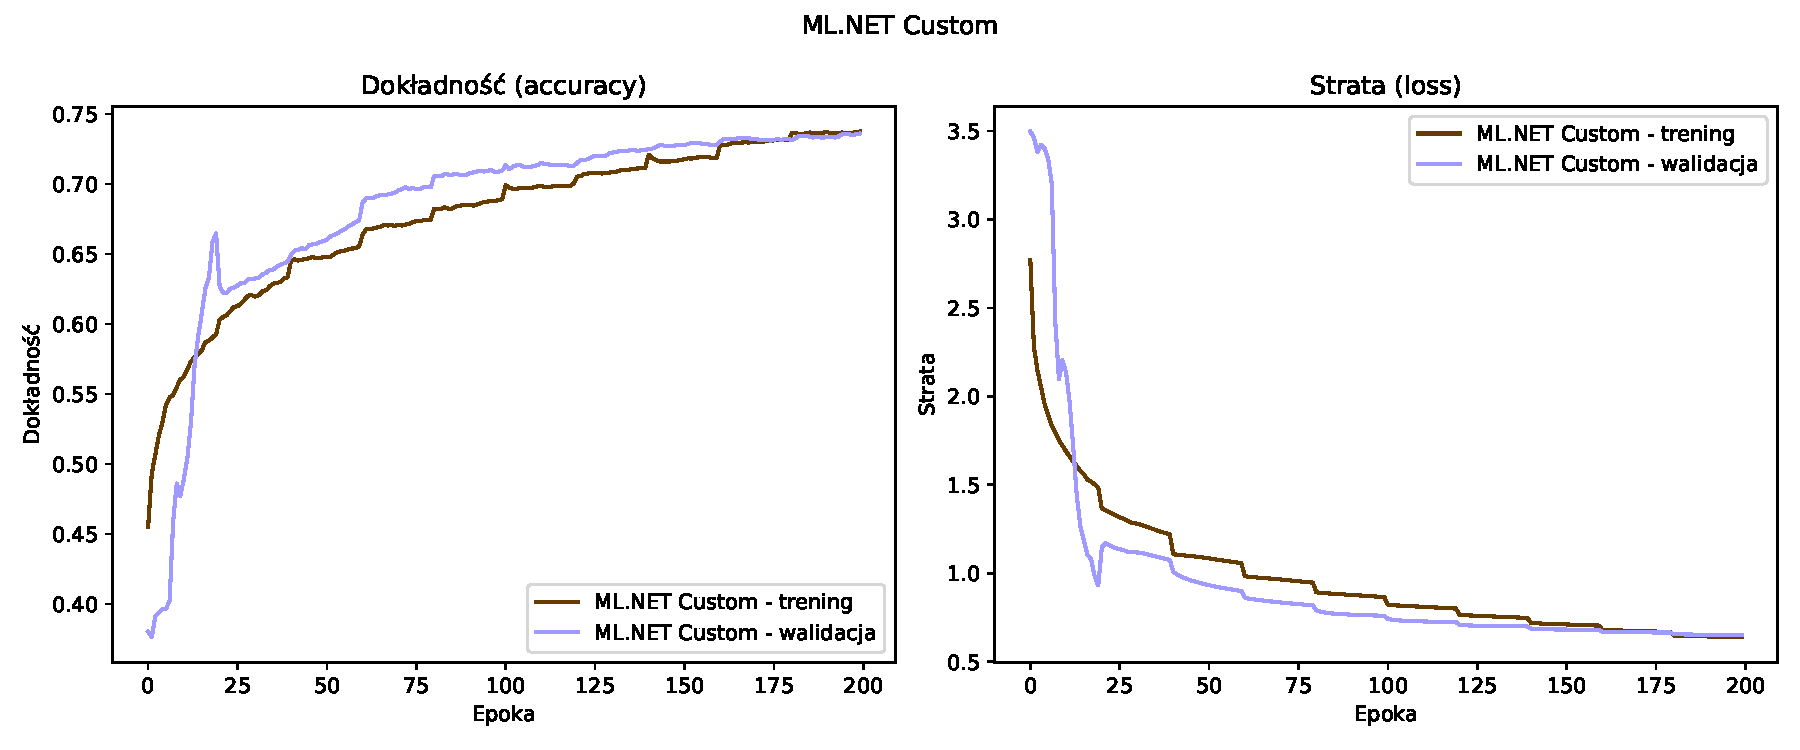
\includegraphics[width=\textwidth]{plot-mlnet-custom-training-overview}
  \caption[Wykresy statystyk modelu ML.NET Custom w trakcie uczenia]{Wykresy dokładności (\emph{accuracy}) oraz straty (\emph{loss}) dla danych testowych i walidacyjnych modelu ML.NET Custom w trakcie uczenia}
  \label{fig:plot-mlnet-custom-training-overview}
\end{figure}

\subsection{Uczenie modelu z użyciem narzędzia ML.NET Model Builder}

\begin{figure}[ht]
  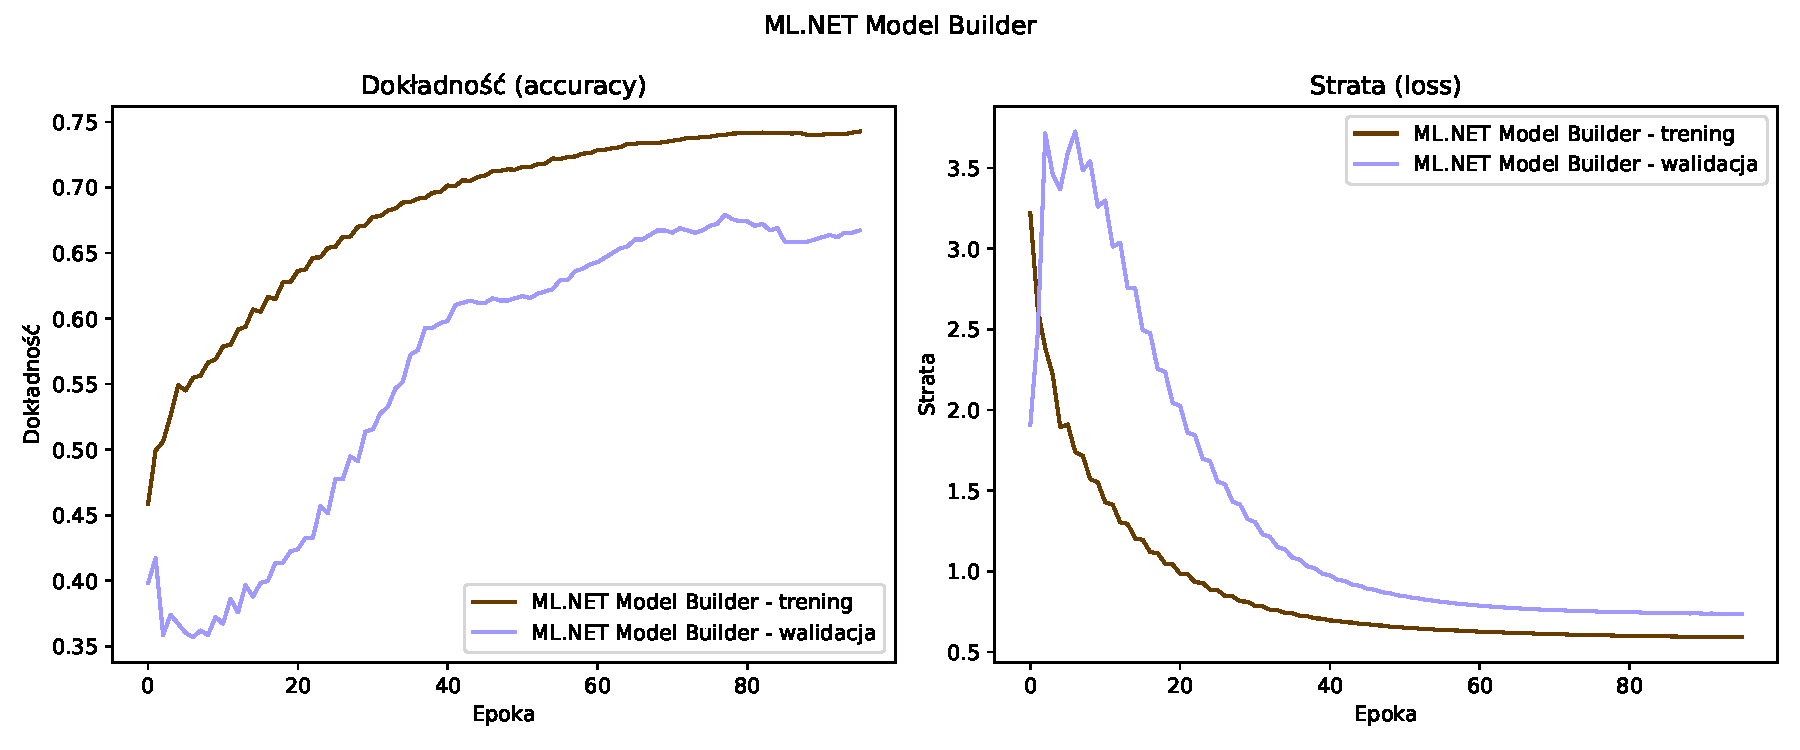
\includegraphics[width=\textwidth]{plot-mlnet-model-builder-training-overview}
  \caption[Wykresy statystyk modelu ML.NET Model Builder w trakcie uczenia]{Wykresy dokładności (\emph{accuracy}) oraz straty (\emph{loss}) dla danych testowych i walidacyjnych modelu ML.NET Model Builder w trakcie uczenia}
  \label{fig:plot-mlnet-model-builder-training-overview}
\end{figure}

\section{Uczenie niestandardowego modelu z użyciem biblioteki TenserFlow.NET}

\begin{figure}[ht]
  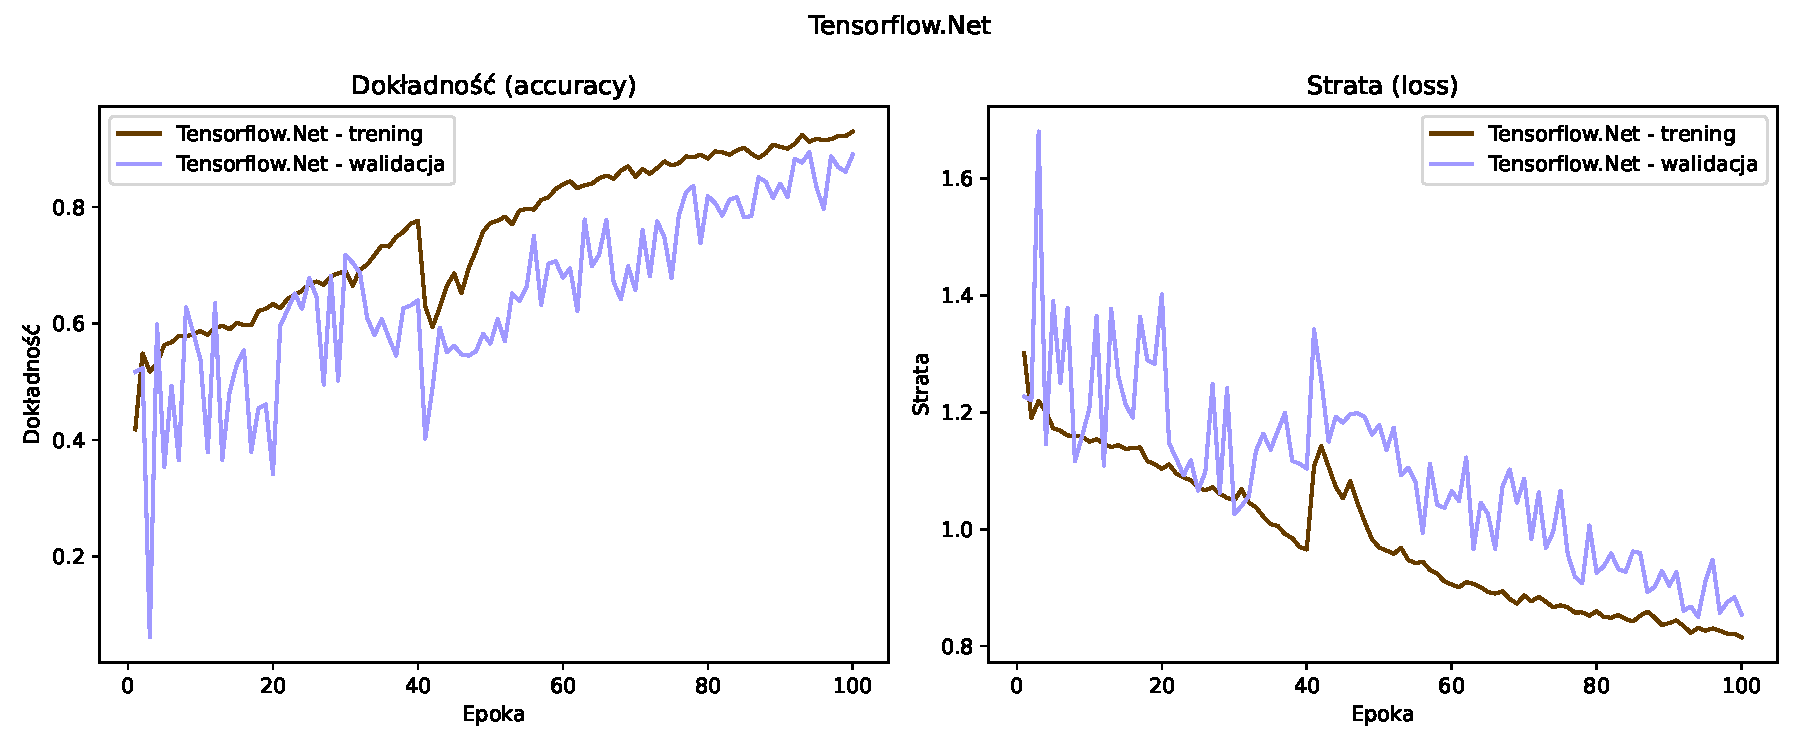
\includegraphics[width=\textwidth]{plot-tensorflownet-training-overview}
  \caption[Wykresy statystyk modelu Tensorflow.NET w trakcie uczenia]{Wykresy dokładności (\emph{accuracy}) oraz straty (\emph{loss}) dla danych testowych i walidacyjnych modelu Tensorflow.NET w trakcie uczenia}
  \label{fig:plot-tensorflownet-training-overview}
\end{figure}

Opis procesu uczenia modelu z użyciem biblioteki TenserFlow.NET

\section{Porównanie wyników}

\begin{figure}[ht]
  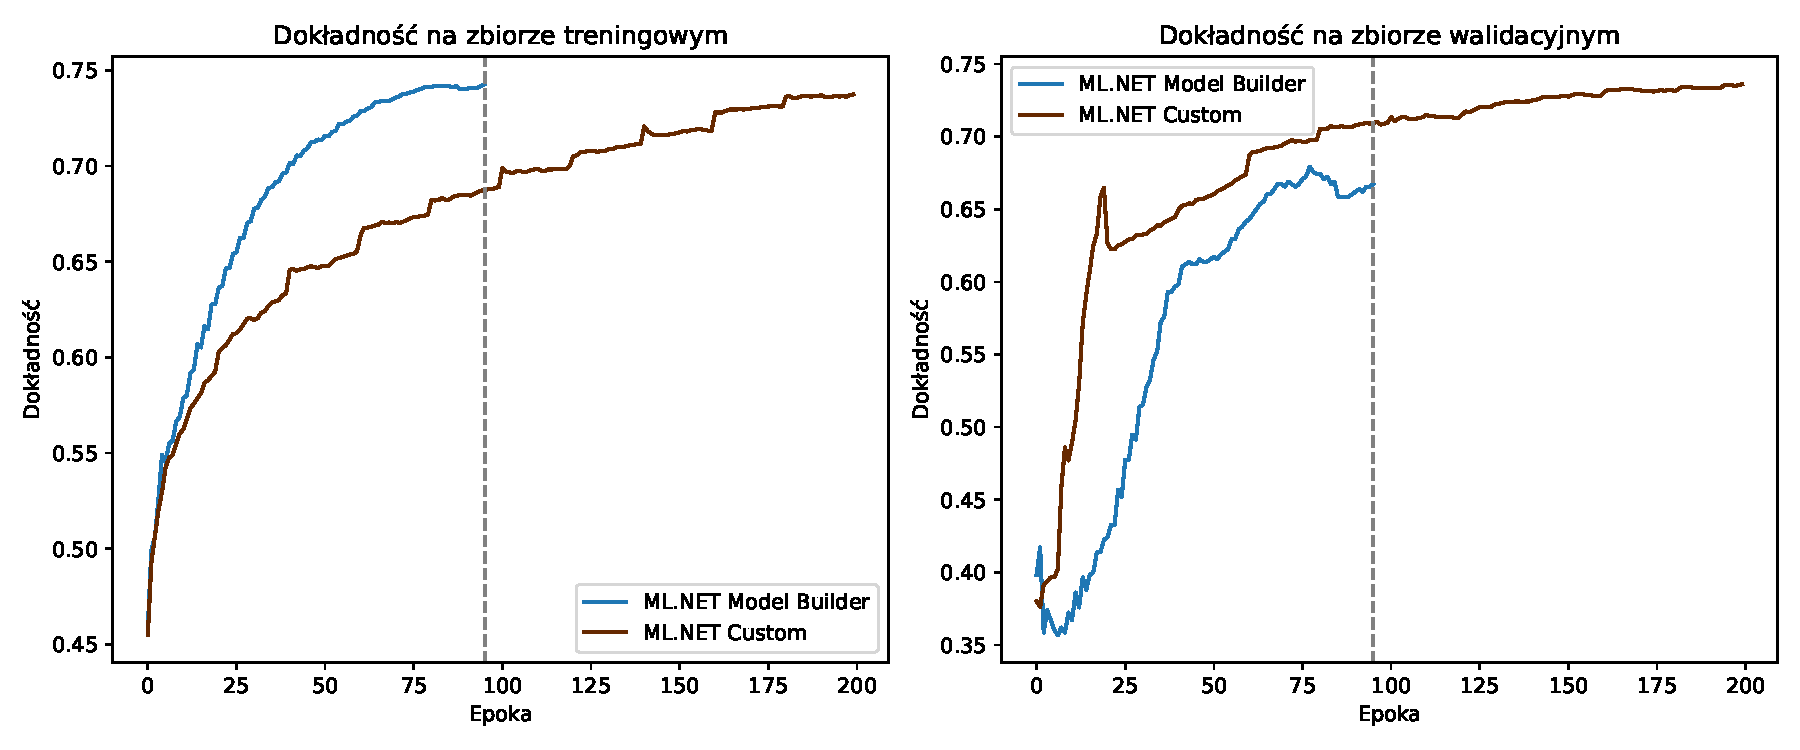
\includegraphics[width=\textwidth]{plot-mlnet-custom-vs-mlnet-model-builder}
  \caption[Porównanie dokładności oraz straty modeli ML.NET Custom oraz ML.NET Model Builder]{Porównanie dokładności (\emph{accuracy}) oraz straty (\emph{loss}) na zbiorze treningowym i walidacyjnym modeli z projektów ML.NET Custom oraz ML.NET Model Builder}
  \label{fig:plot-mlnet-custom-vs-mlnet-model-builder}
\end{figure}

\begin{figure}[ht]
  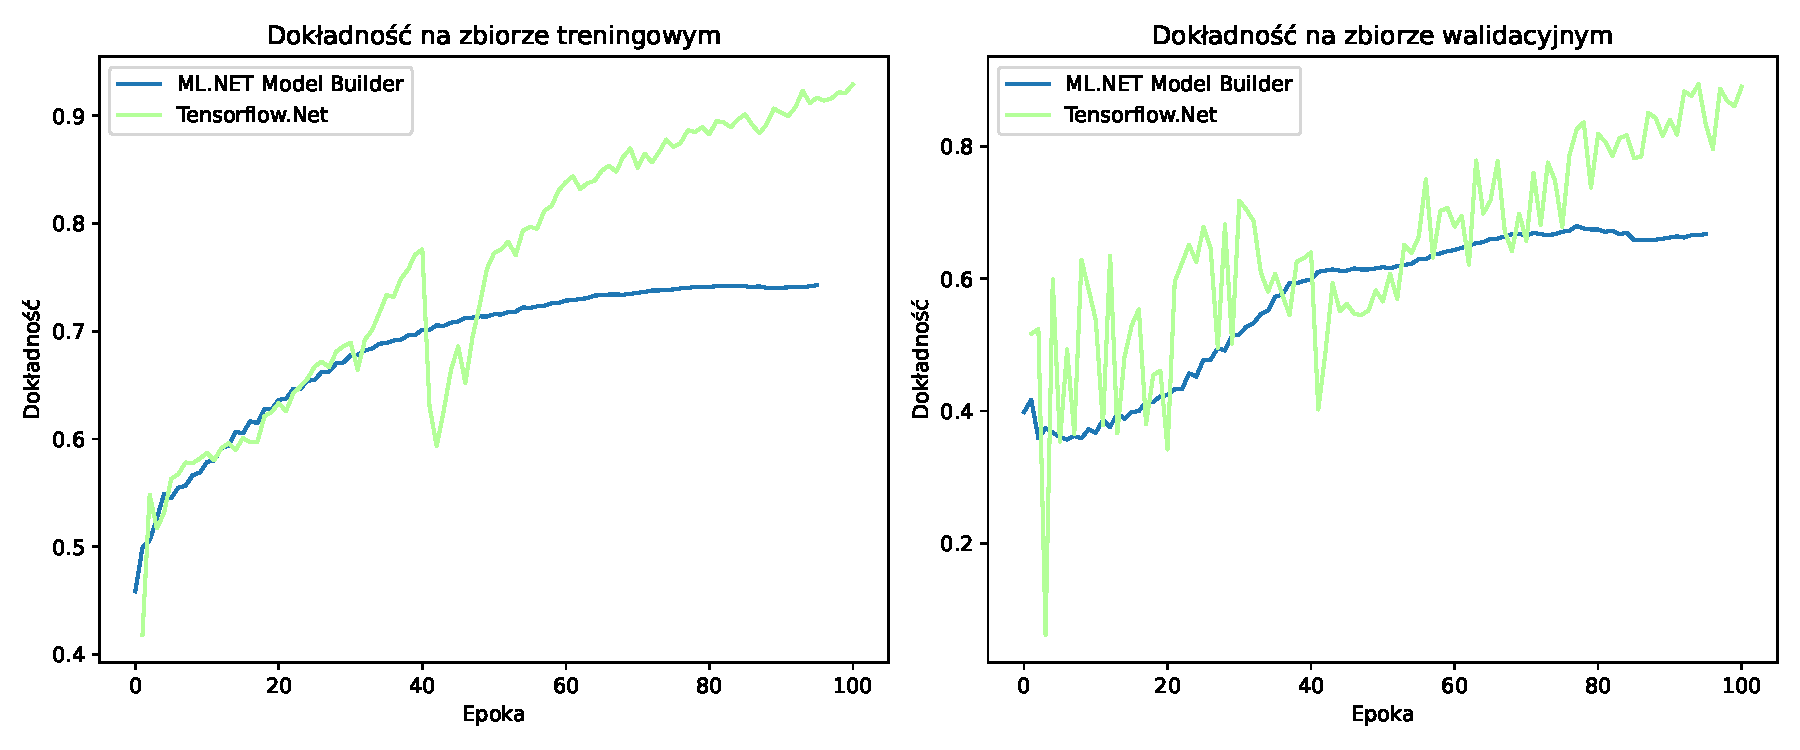
\includegraphics[width=\textwidth]{plot-mlnet-model-builder-vs-tensorflownet}
  \caption[Porównanie dokładności oraz straty modeli ML.NET Model Builder oraz Tensorflow.NET]{Porównanie dokładności (\emph{accuracy}) oraz straty (\emph{loss}) na zbiorze treningowym i walidacyjnym modeli z projektów ML.NET Model Builder oraz Tenserflow.NET}
  \label{fig:plot-mlnet-model-builder-vs-tensorflownet}
\end{figure}

\begin{table}[ht]
  \centering
  \begin{tabular}{|l|r|r|r|r|}
    \hline
                         & \multicolumn{2}{c|}{Zbiór treningowy}                                          & \multicolumn{2}{c|}{Zbiór walidacyjny}                      \\
    \cline{2-5}
                         & \multicolumn{1}{|c|}{Accuracy}        & \multicolumn{1}{|c|}{Loss}             & \multicolumn{1}{|c|}{Accuracy} & \multicolumn{1}{|c|}{Loss} \\
    \hline
    ML.NET Custom        & 0.7373874                             & 0.6378530                              & 0.7359702                      & 0.6511808                  \\
    ML.NET Model Builder & 0.7401715                             & 0.6036751                              & 0.6793103                      & 0.7503802                  \\
    Tensorflow.NET       & 0.9118868                             & 0.8311445                              & 0.8935547                      & 0.8501284                  \\
    \hline
  \end{tabular}
  \caption[Porównanie dokładności oraz straty modeli na zbiorze treningowym i walidacyjnym]{Porównanie dokładności (\emph{accuracy}) oraz straty (\emph{loss}) modeli na zbiorze treningowym i walidacyjnym w epokach szkolenia najlepszych względem na dokładności walidacyjnej}
  \label{tab:train_validation_metric_comparison}
\end{table}

\begin{table}[ht]
  \centering
  \begin{tabular}{|l|r|}
    \hline
                         & \multicolumn{1}{|c|}{Accuracy} \\
    \hline
    ML.NET Custom        & 0.45269742                     \\
    ML.NET Model Builder & 0.70602033                     \\
    Tensorflow.NET       & 0.85926505                     \\
    \hline
  \end{tabular}
  \caption[Porównanie dokładności modeli na tym samym zbiorze testowym]{Porównanie dokładności (\emph{accuracy}) modeli na tym samym zbiorze testowym}
  \label{tab:test_accuracy_comparison}
\end{table}

\section{Wykorzystanie modelu w aplikacji z użyciem biblioteki ML.NET}

W jaki sposób wykorzystać można model w aplikacji
